% CREATED BY DAVID FRISK, 2016
\chapter{Theory}

This section is where the theory behind parsing, the trees and the EM algorithm is described.
\section{Syntax trees}
Explain some basics about syntactic trees and syntactic parsing
\section{GF and Abstract syntax trees}

The type of grammars used in Grammatical Frameworks are a type of \emph{parallel multiple context free grammars} (PMCFG) and are mainly used to describe and formalize the structure of sentences in natural languages. In GF the PMCFG:s for a language in short consists of two parts, the abstract and the concrete part. The abstract part can be seen as a more general form and can be shared between several languages, while the concrete part contains all language specific rules of a language such as vocabulary, morphology and word order. 


The abstract part can be seen as an interlingua called abstact syntax, while the concrete part can be described as a set of rules prescribing how to linearize the abstract syntax to the target language. The abstract syntax can be thought of as \emph{context free grammar} and consists of a set of \emph{symbols} and a set of \emph{production rules}, each rule transforming one symbol to one or several other symbols. These rules can be applied recursively to ultimately produce a set of \emph{terminal symbols}, symbols which can't be further transformed by any production rule. In applications of natural language the terminal symbols can often be seen as words or atomic lexical units and the non-terminal symbols as phrasal structures such as a clause or a verb phrase. The production rules can be seen as a set of universal grammatical rules, for example that a verb phrase could consist of one transitive verb and a noun. The rules and symbols used to obtain a certain set of terminal symbols can be described with a tree structure, and are thus called an \emph{abstract syntax tree}. This tree has an initial symbol as its root node, the intermediate symbols obtained when applying rules as its intermediate nodes and the terminal symbols as its leaf-nodes. 


An example of a chain of production rules used to create a sentence would be one rule transforming the initial symbol \emph{clause} to the intermediate symbols \emph{noun} and \emph{verb phrase}, then another transforming the \emph{verb phrase} to one \emph{transitive verb} and one \emph{noun}, the two \emph{noun}:s and the \emph{transitive verb} might then each be transformed to terminal symbols carrying the meaning of ``horses'', ``eat'' and ``hay'' respectively. This path of production and the associated syntax tree, would carry the meaning of the English sentence ``horses eat hay'' and would indeed produce that sentence when linearizing the abstract syntax using the concrete rules of a properly defined English concrete model. If the abstract model is shared between several languages these terminal symbols will not only represent the English words but the actual meaning behind those words so that in addition to the English ``Horses eat hay'' it also represents the Swedish ``hästar äter hö'' and the Chinese sentence ``ma chi gancao'' (\begin{CJK}{UTF8}{gbsn}马吃干草\end{CJK}). Given the right concrete grammars the abstract syntax tree can thus be linearized to these strings as well. As an example of an abstract syntax tree, figure \ref{fig:ast} shows the tree for this sentence as implemented by the GF standard translation library. It contains more information than the simple one described above but the concept is the same.

\begin{figure}[!htbp]
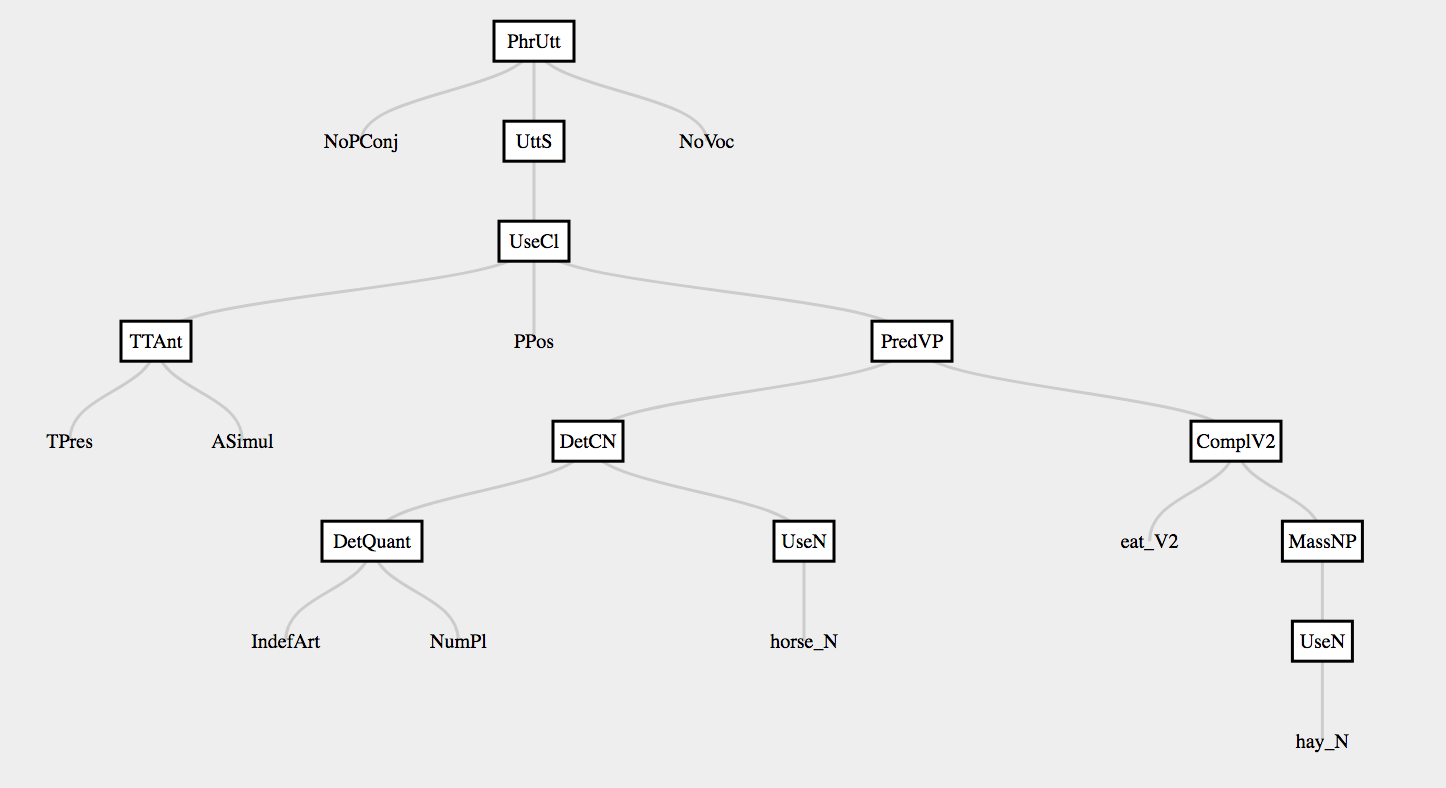
\includegraphics[width=\linewidth]{figure/ast}
\caption{Example of an abstract syntax three from the GF runtime representing the English sentence ``Horses eat hay''.}
\label{fig:ast}
\end{figure}




\section{Probabilistic parsing}
How can we use statistics to disambiguate trees. We need data to estimate probabilities, treebanks are small, we can't just look at text as it is not parsed
\subsection{Context free probabilistic parsing}
PCFG and the equivalent method in in gf
\subsection{Lexicalization and friends}
Lexicalization markovization techniques to include context
\section{UD and Dependency trees}
Difference between dependency and syntax tree, operates on words
\subsection{GF to UD and UD to GF}
Equivalence but not completely, there is ambiguity in ud2gf, needs to be disambiguated.
\section{Expectation Maximization}
Matematical explanation of expectation maximization, problem formulation, what does it do, algorithm description, why does it converge


%\section{Figure}
%\begin{figure}[H]
%\centering
%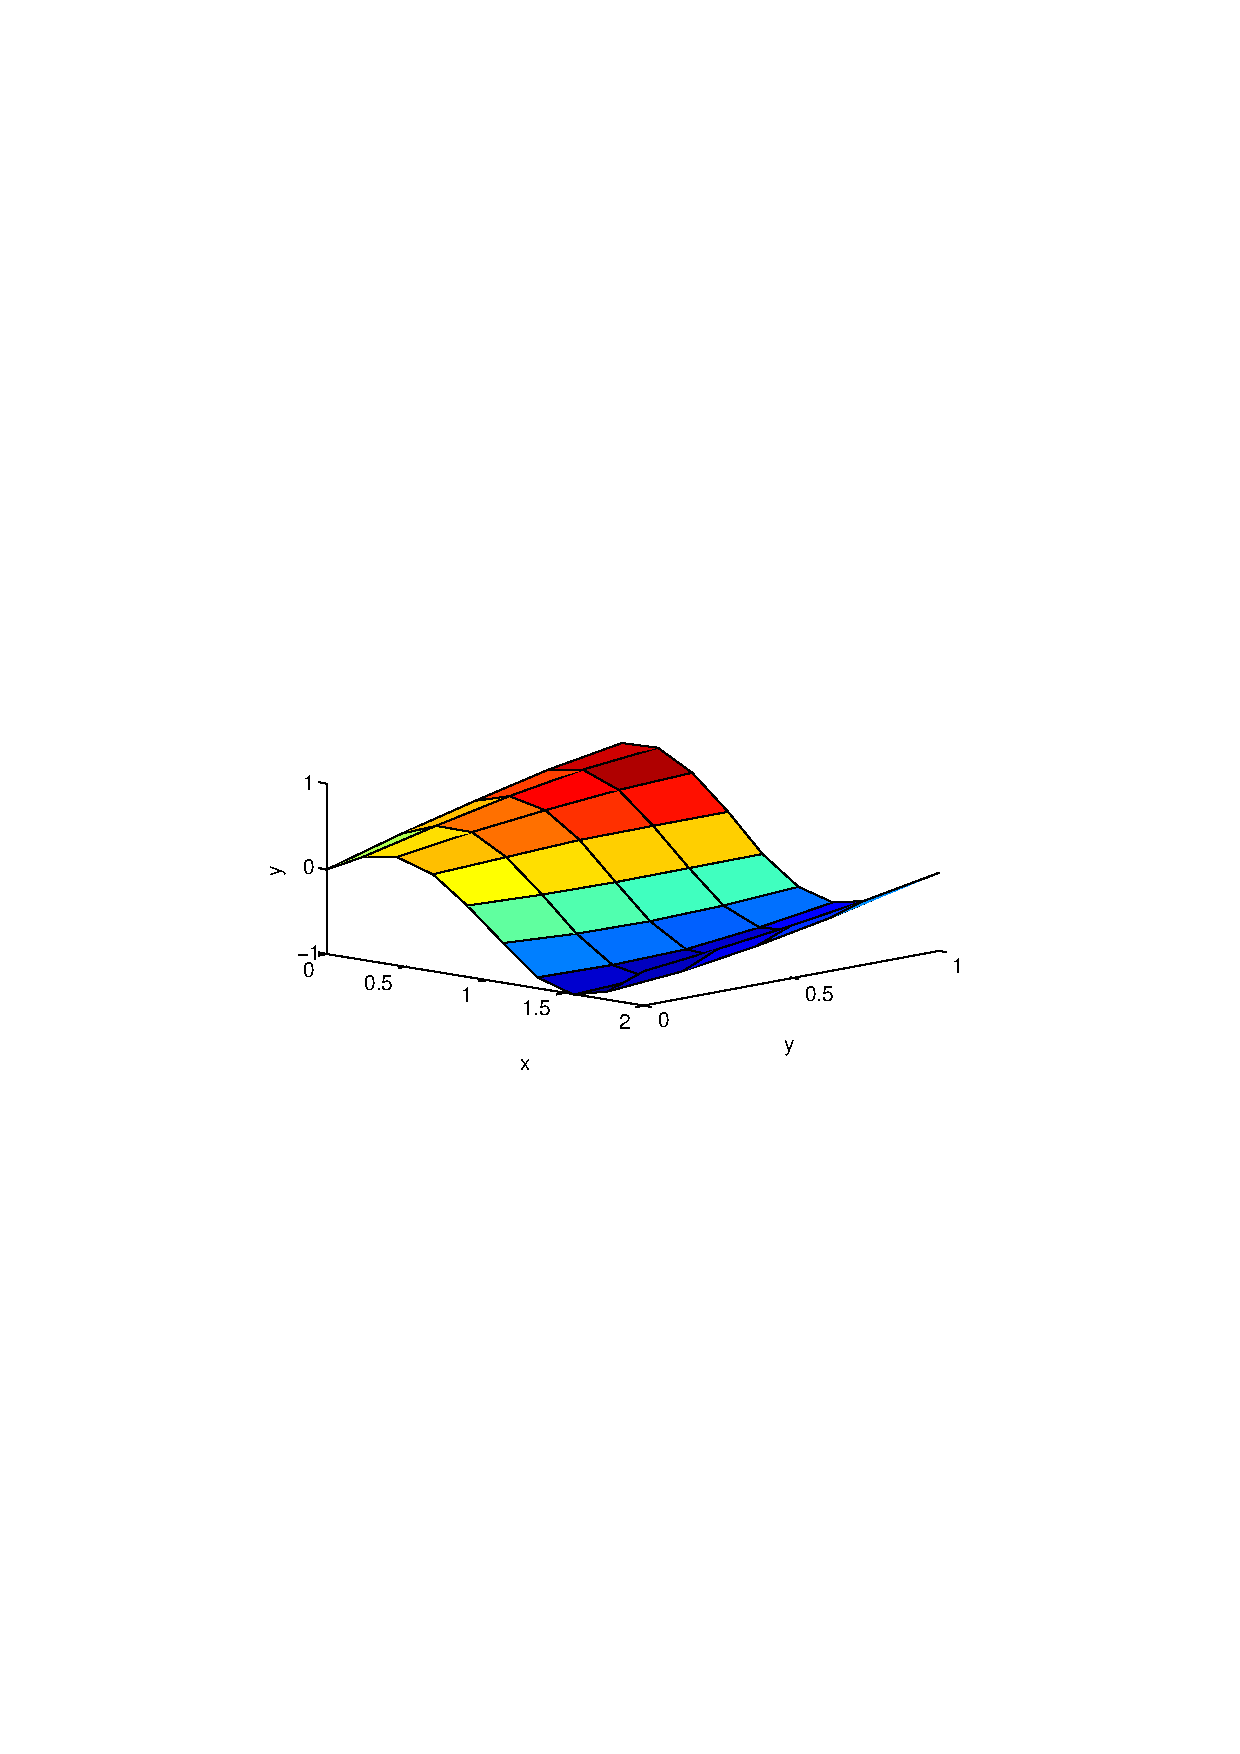
\includegraphics[width=0.45\linewidth, trim=3cm 11cm 3cm 11cm]{figure/X.pdf}
%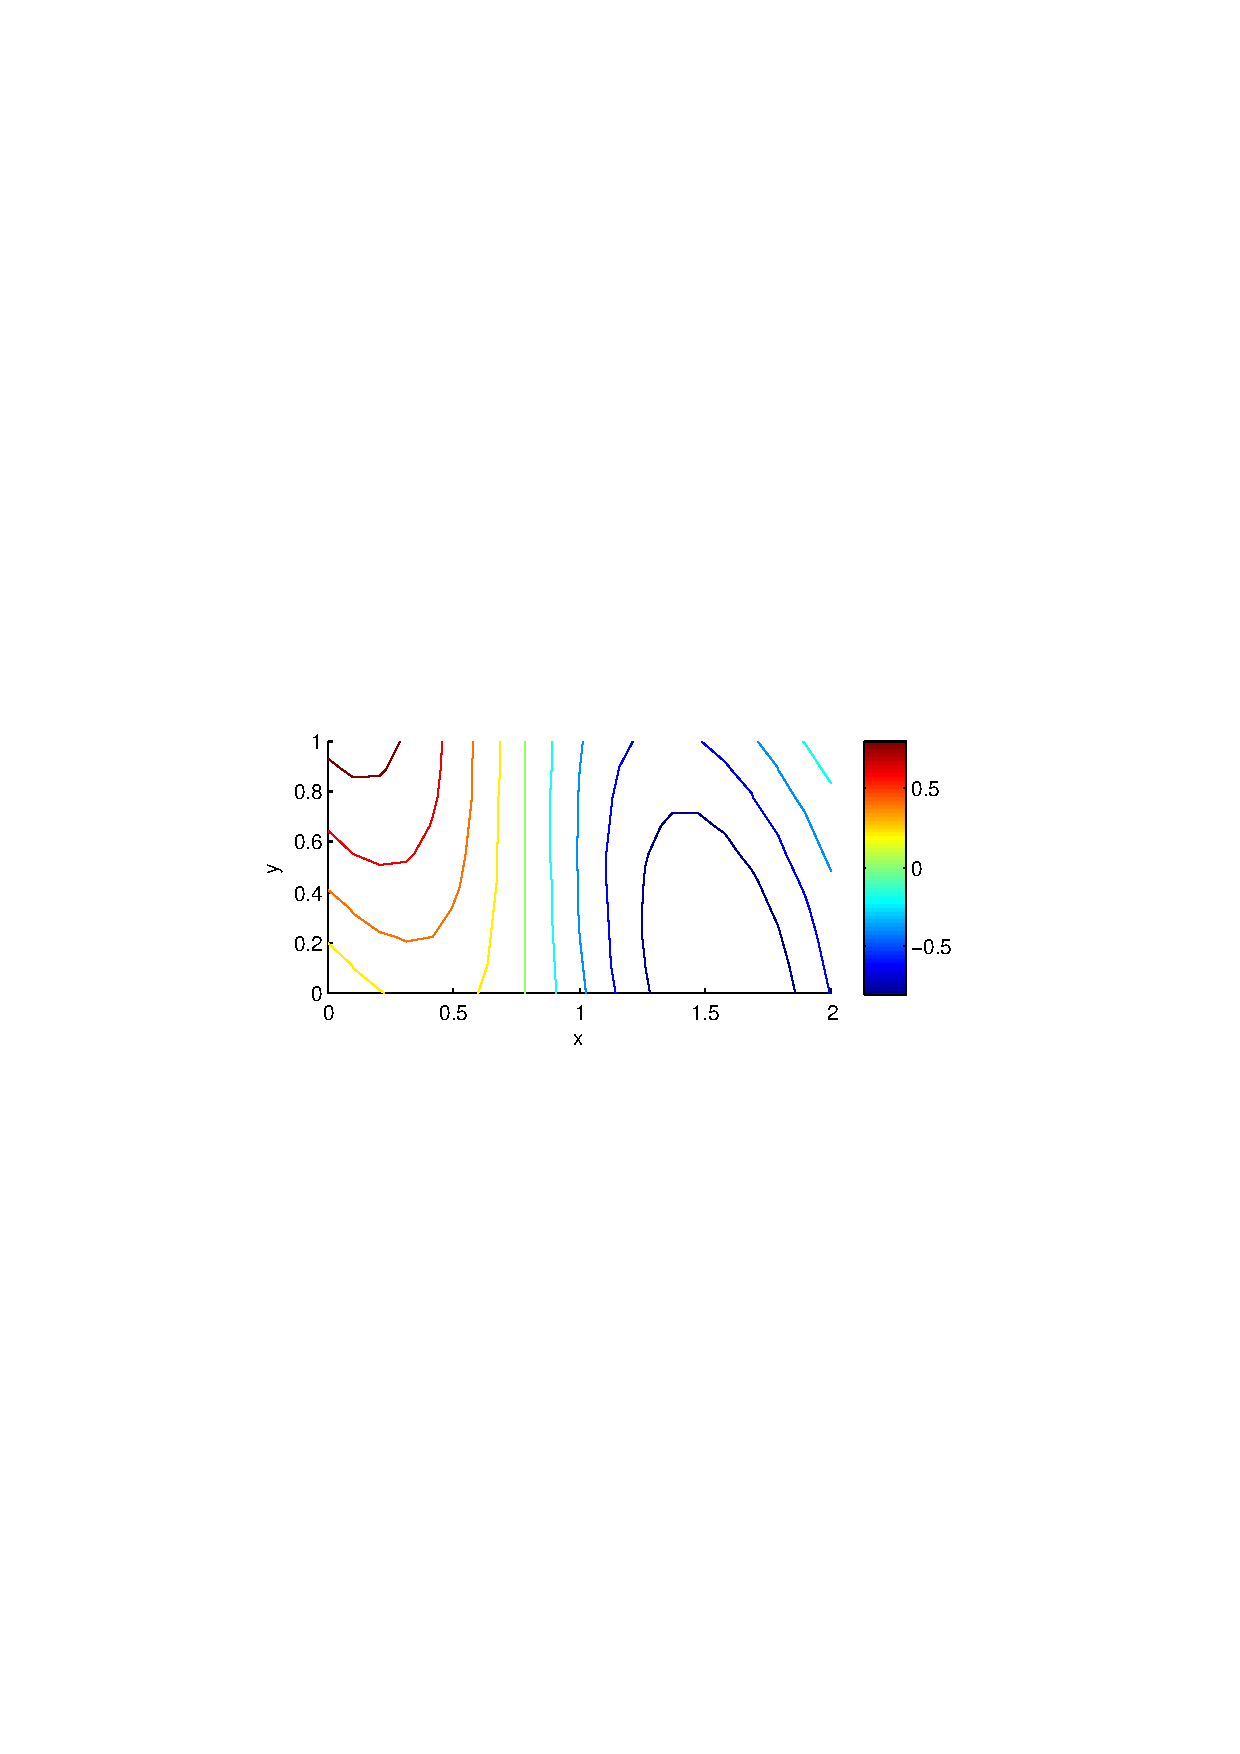
\includegraphics[width=0.45\linewidth, trim=3cm 11cm 3cm 11cm]{figure/Y.pdf}
%\caption{Surface and contour plots showing the two dimensional function $z(x,y)=\sin(x+y)\cos(2x)$.}
%\end{figure}




%\section{Source code listing}
%\begin{minted}[frame=single]{python}
%def em_algorithm(word_counts,
%                 probs,
%                 word_probs,
%                 word_possibilities,
%                 convergence_threshold,
%                 langs):
%    convergence_diff = convergence_threshold
%    expected_counts = dict()
%    expected_fun_counts = dict()
%    
%\end{minted}
